\documentclass[11pt,a4paper]{article}
\usepackage[margin=25mm]{geometry}
\usepackage[T1]{fontenc}
\usepackage[utf8]{inputenc}
\usepackage{lmodern,amsmath,amssymb,amsthm,mathtools,booktabs,array,graphicx,microtype}
\usepackage{xcolor,hyperref,xurl}
\hypersetup{colorlinks=true,linkcolor=blue,citecolor=blue,urlcolor=blue,
 pdftitle={Shape Continuation for Convex-Polytope Packing},
 pdfauthor={Yohei Nakajima and Alejandro Zarzuelo Urdiales}}
\setlength{\emergencystretch}{2em}
\makeatletter
\setlength{\@fptop}{0pt}
\setlength{\@fpsep}{20pt}
\setlength{\@fpbot}{0pt plus 1fil}
\makeatother
\newcommand{\R}{\mathbb R}
\newcommand{\Q}{\mathbb Q}
\newcommand{\B}{\mathbb B}
\newcommand{\conv}{\operatorname{conv}}
\newcommand{\SO}{\operatorname{SO}}
\newcommand{\vol}{\operatorname{vol}}
\newcommand{\code}[1]{\texttt{\nolinkurl{#1}}}
\newcommand{\repo}{https://github.com/alejandrozu/platonic-packing}
\newcommand{\frozen}{https://github.com/alejandrozu/platonic-packing/tree/1abc63218db34cea95802aeb3b6d4a6b6fe1c61b}
\newcommand{\blob}{https://github.com/alejandrozu/platonic-packing/blob/1abc63218db34cea95802aeb3b6d4a6b6fe1c61b}
% Filled only from successful, source-hashed, axiom-audited Lean build receipts.
\newcommand{\leanRecords}{402}
\newcommand{\leanCubeRecords}{99}
\newcommand{\leanNDRecords}{303}
\newcommand{\leanFourDRecords}{195}
\newcommand{\leanFiveDRecords}{62}
\newcommand{\leanSixDRecords}{46}
\newcommand{\leanPieces}{10,796}
\newcommand{\leanPairs}{235,462}
\newcommand{\leanAlgebraicRecords}{130}
\newcommand{\leanAlgebraicFamilies}{130}
\newtheorem{proposition}{Proposition}
\newtheorem{theorem}{Theorem}
\title{Shape Continuation for Convex-Polytope Packing:\\Generalization and Lean-Verified Catalogue Certificates}
\author{Yohei Nakajima \and Alejandro Zarzuelo Urdiales}
\date{16 October 2026}
\begin{document}
\maketitle
\begin{abstract}
We generalize soft-to-rigid finite-container packing from polygons and cubes to convex polyhedra and regular polytopes in dimensions four through six. Two paths are distinguished: blending with an inscribed ball, and erosion followed by dilation, which retains an actual eroded core for non-tangential solids. Continuation becomes one move in an archive search alongside symmetry-released starts, insertion, deletion, rigid perturbation, crystal cuts and nested substitution. A new Lean development proves dimension-independent certificate soundness and verifies all \leanRecords{} selected rational certificates plus \leanAlgebraicRecords{} additional algebraic-coordinate witnesses, covering all 140 frozen problem families in dimensions 3--6. The kernel checks exported raw rotation parameters, proper rotations, congruence, whole-body containment and every pairwise separation. Further theorems establish an exact support-function identity, orientation attenuation and quantitative clearance guarantees under perturbation. A separate source audit binds these exact literals to the original records without changing scales or placements; parsing remains outside the kernel. The additional cohort selects one two-piece witness per remaining family; this is family coverage, rather than verification of every population in the 10,398-witness archive. Independent exact-arithmetic checkers and five separately rechecked examples complement this formal layer. A historical comparison of 1,824 attempts on 40 prism-family cases illustrates why improvement frequency and magnitude lead to different search policies. The results establish constructive feasibility and an auditable method; they do not prove global optimality or universal superiority of continuation.
\end{abstract}

\section{Purpose and relation to earlier work}
Finite packing asks how small a prescribed container can be while holding a fixed number of congruent bodies. It combines discrete contact patterns with continuous translations and rotations. A numerical optimizer may locate an attractive configuration while leaving imperceptible overlaps; a reliable constructive bound therefore needs a separate validity argument.

Nakajima's soft-to-rigid study~\cite{nakajima2026} uses gradual shape change as an alternative search path. Its controlled comparisons favor tuned rigid starts overall, while showing complementary behavior on particular polygon instances. Section 7 already credits Zarzuelo's extension to Platonic solids, generalized exact checking and repeated softening of archived packings. That downstream use motivates the present account. We do not present the broader catalogue as an independent controlled validation of the original simulator.

The earlier DOI publications document the initial nine-family implementation~\cite{zarzueloMethods}, structural analysis of its 351 constructions~\cite{zarzueloPatterns}, and the associated data release~\cite{zarzueloData}. The present paper concerns a later, substantially larger implementation in the shared repository~\cite{archive}. Its contributions are the geometric distinction needed for non-tangential 3D solids, the supported higher-dimensional search and certification pipeline, the integration of multiple construction families into one archive, and a new, explicitly bounded Lean proof layer. The three earlier DOI objects identify the original scientific and data record; their frozen dataset must not be confused with the expanded snapshot below.

General polyhedron packing and continuous rotations predate this work~\cite{romanova2018}; Berthold et al.~\cite{berthold2026} already studied all 25 ordered Platonic-solid pairs. Rounded polyhedral particles and shape evolution also have established uses~\cite{jin2015}. Sequential linear programming~\cite{torquato2010}, lattice packing~\cite{betke2000}, and periodic polyhedron packing~\cite{torquato2009} supply important context and seed constructions. We claim an implemented and inspectable generalization of a search-and-certification pipeline, rather than invention of these underlying geometric ideas.

The repository is an open, versioned research archive connecting independent contributions with geometry definitions, coordinate witnesses, certificates, source lineage and search code. Its literature review and historical-source audit~\cite{repoRelated,repoAudit} connect the catalogue to prior research; its search-method study, large-population analysis and higher-dimensional notes~\cite{repoSearch,repoLarge,repoHigher} record the implementation's empirical development. These project research materials complement, rather than replace, citations to the original papers.

\section{Packing problem and normalization}
Fix an integer $d\geq1$. Let $P,C\subset\R^d$ be compact, full-dimensional convex polytopes, with fixed reference scales and the origin in their interiors. Write
\begin{equation}
\begin{split}
s^*_{P\to C}(n)=\inf\{s>0:\;&p_i+R_iP\subseteq sC,\quad R_i\in\SO(d),\\
&\operatorname{int}(p_i+R_iP)\cap\operatorname{int}(p_j+R_jP)=\varnothing
\quad(i\ne j)\}.
\end{split}
\end{equation}
A common container translation can be absorbed into the piece centers. Requiring proper rotations matters for chiral solids: a reflected enantiomer is not generally a rotated copy.

For unit-edge solids, $s$ is container edge divided by piece edge. Catalan self-packings use a fixed canonical polar-dual shape; elongated prisms retain their specified aspect ratio. For mixed shapes, equal numerical edge ratios need not imply equal density. With compatible reference volumes,
\begin{equation}\label{eq:density}
\eta=\frac{n\vol_d(P)}{s^d\vol_d(C)},\qquad
s\geq\left(\frac{n\vol_d(P)}{\vol_d(C)}\right)^{1/d}.
\end{equation}
The exponent changes with dimension; $n^{1/d}$ alone is appropriate only when the reference volumes agree. Defining $\sigma=s[\vol_d(C)/\vol_d(P)]^{1/d}$ gives $\eta=n/\sigma^d$.

Native higher-dimensional coordinates need an additional conversion. If $P_0,C_0$ have canonical edge lengths $e_P,e_C$, let $\mu=e_P/e_C$. A record at edge ratio $s$ places copies of $P_0$ in
\begin{equation}\label{eq:native}
c_C+s\mu C_0.
\end{equation}
Consequently raw canonical volumes give
$\eta=n\vol_d(P_0)/[(s\mu)^d\vol_d(C_0)]$. Omitting $\mu$ can reverse comparisons. Likewise, comparisons with circumradius-normalized literature require the corresponding edge conversion.

\section{Two continuation paths}
Let $\B_d$ be the closed unit Euclidean ball and assume $\rho\B_d\subseteq P$, $\rho>0$.

\subsection{Homothetic-core blending}
For $0\leq\tau\leq1$, set
\begin{equation}\label{eq:blend}
H_\tau=(1-\tau)P\oplus\tau\rho\B_d.
\end{equation}
Here $\oplus$ denotes Minkowski addition. The endpoints are $H_1=\rho\B_d$ and $H_0=P$. This formula is dimension-independent and does not require all facets to touch the inscribed ball.

\begin{proposition}\label{prop:blend}
The family satisfies $H_\tau\subseteq P$. If $0\leq\tau_1\leq\tau_2\leq1$, then $H_{\tau_2}\subseteq H_{\tau_1}$.
\end{proposition}
\begin{proof}
Every point of $H_\tau$ is a convex combination of a point of $P$ and a point of $\rho\B_d\subseteq P$. For a unit direction $u$, its support function is
\[
h_{H_\tau}(u)=(1-\tau)h_P(u)+\tau\rho.
\]
Since $h_P(u)\geq\rho$, this expression decreases with $\tau$. Support-function comparison gives the claimed inclusion.
\end{proof}

Containment is formalized in Lean as \code{convex_blend_subset}. The theorem \code{convexBlend_antitone} proves the nesting inclusion directly by convex combinations. It applies to every convex target and every inscribed body; tangency and regularity are unnecessary. A separate support-function development now proves the extent identity used above.

\subsection{Exact support identity and orientation attenuation}\label{sec:supportidentity}
For nonempty compact $P\subseteq\R^d$, write
$h_P(u)=\sup_{x\in P}\langle u,x\rangle$.
The ball-blend identity used in Nakajima's method~\cite[Section 3]{nakajima2026}
holds in every finite dimension and for every direction:
\begin{theorem}\label{thm:supportblend}
If $0\leq\tau\leq1$ and $\rho\geq0$, then
\begin{equation}\label{eq:supportblend}
h_{H_\tau}(u)=(1-\tau)h_P(u)+\tau\rho\|u\|.
\end{equation}
For proper rotations $R,S\in\SO(d)$,
\begin{equation}\label{eq:orientationattenuation}
\big|h_{R H_\tau}(u)-h_{S H_\tau}(u)\big|
=(1-\tau)\big|h_{RP}(u)-h_{SP}(u)\big|.
\end{equation}
\end{theorem}
\begin{proof}
A linear functional attains its maximum on nonempty compact $P$. Its maximum
on the radius-$\rho$ ball is $\rho\|u\|$, including $u=0$. Nonnegative linear
combinations of these maximizers both attain and bound the support of their
Minkowski blend, proving~\eqref{eq:supportblend}. Orthogonal transformations
preserve the ball and send a direction to its inverse image. The ball terms
therefore cancel between $R$ and $S$; $1-\tau\geq0$ gives the absolute-value identity.
\end{proof}

\code{SupportIdentity.lean} defines the genuine real support supremum and
proves maximum attainment before using it. Its theorems
\code{support_ballBlend}, \code{support_rotated_ballBlend} and
\code{orientation_support_abs_difference} establish these statements in real
inner-product spaces, with an explicit \code{euclidean_support_ballBlend}
specialization for every $d$. The algebraic identity itself needs neither
convexity nor an inscribed-ball assumption; those are separate hypotheses for
$H_\tau\subseteq P$. The proof applies to orthogonal isometries, hence in
particular to the proper rotations permitted by a packing. At $\tau=1$ the
support is orientation-independent. This is an exact statement about geometric
extent, not a scaling law for the full search energy or its gradients, and does
not prove that deferred orientation improves optimization.

\subsection{Actual eroded cores for non-tangential solids}
For a radius $r\geq0$, define the erosion and opening
\begin{equation}\label{eq:opening}
E_r=P\ominus r\B_d=\{x:x+r\B_d\subseteq P\},\qquad
O_r=E_r\oplus r\B_d.
\end{equation}
If $P=\{x:a_f\cdot x\leq b_f,\ f=1,\ldots,F\}$ with unit outward normals, then
\begin{equation}\label{eq:erosionfacets}
E_r=\{x:a_f\cdot x\leq b_f-r,\ f=1,\ldots,F\}.
\end{equation}
This uses the actual supporting planes. For general $P$, it does \emph{not} imply $h_{E_r}(u)=h_P(u)-r$ in every direction: vertices and active facets can change.

\begin{proposition}\label{prop:opening}
For $0\leq r\leq R$, $O_R\subseteq O_r\subseteq P$, and $O_0=P$.
\end{proposition}
\begin{proof}
By definition, $y+z\in P$ whenever $y\in E_r$ and $z\in r\B_d$, proving $O_r\subseteq P$. If $R>0$ and $x=y+Ru$ with $y\in E_R$, $\|u\|\leq1$, write
$x=[y+(R-r)u]+ru$. For $\|v\|\leq1$, the point
$y+(R-r)u+rv$ belongs to $y+R\B_d\subseteq P$ by the triangle inequality. Thus $y+(R-r)u\in E_r$ and $x\in O_r$. The case $R=0$ and the endpoint follow directly.
\end{proof}

Lean's \code{minkowskiOpening_subset} proves opening containment for any structuring body. The new \code{ballOpening_antitone} and \code{ballOpening_zero} prove the radius nesting and rigid endpoint in Proposition~\ref{prop:opening}. These statements hold in arbitrary real normed vector spaces, including every finite-dimensional Euclidean space, and do not require convexity of $P$.

For a tangential polytope with every unit-normal offset equal to $\rho$, equation~\eqref{eq:erosionfacets} gives
$E_r=(1-r/\rho)P$ for $0\leq r<\rho$. Hence $O_r=H_{r/\rho}$ on that interval. The distinction matters for prisms with unequal facet distances and for many Archimedean solids: uniform core scaling and true erosion are different paths even though both can stay inside $P$.

The generalized 3D implementation precomputes the eroded core numerically, tracking its changing combinatorics. Sampling and bisection locate transitions; this preprocessing is not an exact proof of every intermediate body. Internal search units set the inradius to $1/2$ and cap the non-tangential erosion radius at $0.49$, before a possibly degenerate core. The initial body is therefore rounded but need not be a sphere. The supported regular 4D--6D polytopes are tangential and use the homothetic-core formula; the implementation is not an arbitrary-dimensional erosion engine. Final rigid certificates are independent of these intermediate approximations.

\subsection{A geometric generalization to every finite dimension}
For each $d\in\mathbb N$, instantiate the formal statements in \code{EuclideanSpace} $\R\,(\operatorname{Fin}d)$, whose norm is Euclidean. The named theorem \code{euclidean_ball_continuation} proves the nested family and exact rigid endpoint for every $d$, rather than checking a list of dimensions. The distinction of norm is essential: the default norm on an unwrapped coordinate function space is a supremum norm, whose balls are boxes.

The theorem \code{euclidean_opening_preserves_packing} transports these inclusions through each piece's individual placement. A feasible rigid packing therefore gives feasible softened packings, in every finite dimension. Hardening an arbitrary soft configuration can create overlaps; neither this theorem nor the search algorithm guarantees that those overlaps can always be removed. Proper rotations of the actual certificate placements are proved separately. Thus the formal dimension generalization establishes the geometry and certificate interface, while convergence and intermediate numerical erosion remain distinct questions.

\section{From one continuation to an archive search}
\subsection{Candidate generation and tightening}
The search separates three jobs: generate a promising configuration, reduce its scale numerically, and validate a final exact witness. Soft dynamics minimize squared positive overlap and wall penalties together with inward pressure. Momentum, bounded pose updates and annealed noise help the rounded pieces rearrange. Softness decreases to zero, followed by hard settling. Quaternion orientations are used in 3D. In dimension $d$, skew-matrix increments supply the $d(d-1)/2$ local rotation parameters, with numerical matrices periodically reorthonormalized.

For 3D rounded cores, contact calculations combine separating-axis penetration tests and distances between disjoint features. In higher dimensions, support-point queries and optimized separating hyperplanes avoid treating 3D edge-cross-edge axes as a complete $d$-dimensional test. These are search calculations; their numerical residuals are not feasibility proofs.

A legalizer spreads centers if necessary, finds candidate separating planes and refits the container including its translation. Constrained tightening then minimizes scale using vertex/wall and pair-plane constraints. Sequential linear programming uses trust regions and optional regularization; an earlier constrained nonlinear path remains available. Tightening can fail, stagnate or miss an improved basin. The program name \code{exact.py} refers to the geometric formulation and does not make its numerical optimization exact arithmetic.

\subsection{Reusing and changing arrangements}
The archive stores selected witnesses and pools of distinct useful arrangements for each problem and population. A hop slightly expands and perturbs an existing packing, optionally softens a cluster or all pieces, then hardens and tightens. This gives continuation a role beyond a new random start. Related remelting and insertion were also explored in the independent cube continuation by \code{@BuilderOfAgents}/tronford~\cite{tronford}; these moves are not claimed as originating here. An insertion move starts from $n-1$ pieces, deletion starts from $n+1$, and reinsertion removes a small set before searching for better holes. Cheap rigid perturbation followed by tightening competes with soft moves.

Deleting pieces preserves feasibility, giving
\begin{equation}\label{eq:monotone}
s^*_{P\to C}(n)\leq s^*_{P\to C}(n+1).
\end{equation}
The archive propagates useful deletions and retains their lineage. A plateau in selected bounds may result from deleting a loosely constrained piece; it is not by itself a plateau theorem for the unknown optimum.

Adaptive allocation uses measured improvements, logarithmic scale gains, elapsed time, failure streaks, adjacent populations and plateau information. Exploration and polishing use different policies. Such heuristics help distribute finite computation, but no convergence guarantee is asserted.

\subsection{Symmetric starts and finite crystal cuts}
In 3D, \code{symfresh} creates orbits under a randomly selected cyclic symmetry of the container during the soft phase, then releases the symmetry before unrestricted tightening. A structured start can reduce an unproductive search space while allowing the final packing to break the imposed symmetry. A symmetric seed and a symmetric final witness are therefore distinct observations. Higher-dimensional symmetric starts also use central inversion, reflections and suitable four-element groups, while the exported pieces must still have proper rotations.

Grid, lattice, double-lattice and prism-column arrangements give further seeds. Finite windows are cut from periodic constructions, translated and rotated relative to the container, then refitted and tightened. Prior lattice and dense-periodic work~\cite{betke2000,torquato2009,jiao2011} supplies context. A high infinite-volume density does not guarantee a good small finite cut: wall compatibility and missing boundary cells can dominate. Conversely, a good finite-container packing is not evidence of a physically selected crystal or a densest infinite packing.

\subsection{Nested substitution and community lineage}
Suppose $m$ copies of $P$ fit in $aQ$ and $k$ copies of $Q$ fit in $bC$, all in compatible units. If inner poses are $R_ix+p_i$ and outer poses are $U_jy+q_j$, scale the whole outer arrangement by $a$ and replace each outer piece by the inner packing. The resulting poses are
\begin{equation}\label{eq:compose}
U_jR_ix+U_jp_i+a q_j\quad\hbox{in }abC.
\end{equation}
Thus any subset of the $mk$ pieces proves
\begin{equation}\label{eq:composebound}
s^*_{P\to C}(N)\leq ab,\qquad 1\leq N\leq mk.
\end{equation}
This classical inclusion principle needs dimension and normalization compatibility. Container-center translations must be handled before composing poses. Boundary contacts remain legal for the mathematical packing problem; the production exporter subsequently adds clearance and rechecks its constructed witness.

The implemented 3D sweep currently uses Platonic intermediate solids; the higher-dimensional sweep uses the supported regular polytopes. It generalizes the project's whole-body inclusion contribution by PingYou Ltd~\cite{ping79}; related independent contributions include honeycomb windows, prism subdivisions and face lifts~\cite{pingConstructions}. These construction ideas and inherited coordinates retain their original attribution. Re-padding, exact checking or combining a witness does not transfer its construction authorship. Lean's affine transport and subset-replacement lemmas formalize ingredients of this inclusion reasoning, rather than an end-to-end proof of either composition script or all instances of~\eqref{eq:composebound}.

Other contributions include Stian's octahedron-in-cube improvements for $n=13,15,18$~\cite{stian}; konoha-ily2's exact rational cube witnesses~\cite{konoha}; Ryan Xu's independently published cube coordinates for $n=34,35,36$~\cite{ryan}; and Sam Scott's tightening audit of Haowei Lin's previously published arrangements~\cite{scott}. The archive also incorporates coordinate reconstructions matching Friedman's historical $n=13,14$ cube bounds by \code{@BuilderOfAgents}/tronford~\cite{builderRecon}, alongside original sources from Friedman, Walsh, Lin and Berthold et al., documented in the source audit~\cite{repoAudit}. Imported original constructions, reconstructions and later refinements remain separate provenance roles. The catalogue is the combined result of these searches and contributions, not solely the work of the two manuscript authors.

\section{Exact witnesses and the scope of formal proof}
\subsection{Finite geometric certificate}
Write $V_i$ for the transformed vertex set of piece $i$ and let the container be an intersection of closed halfspaces. A sufficient certificate consists of
\begin{align}
a_f\cdot v&\leq b_f &&(v\in V_i,\ \hbox{all }i,f),\label{eq:walls}\\
u_{ij}\cdot v&\leq\ell_{ij}<r_{ij}\leq u_{ij}\cdot w
&& (v\in V_i,\ w\in V_j,\ i\ne j).\label{eq:pairs}
\end{align}
The wall offsets incorporate the scale and center of the container. Strict margins may also be required at walls. Nonzero pair normals and a positive separating gap are implicit in~\eqref{eq:pairs} whenever both vertex sets are nonempty.

\begin{theorem}\label{thm:certificate}
If~\eqref{eq:walls}--\eqref{eq:pairs} hold, every convex hull $\conv V_i$ lies in the container and these closed convex hulls are pairwise disjoint.
\end{theorem}
\begin{proof}
A linear inequality valid at all vertices is valid on every convex combination. Consequently each hull satisfies every wall inequality. A common point of two hulls would have its projection at once at most $\ell_{ij}$ and at least $r_{ij}$, contradicting $\ell_{ij}<r_{ij}$.
\end{proof}
This is a dimension-independent statement. To conclude that these hulls represent congruent copies of the intended solid, one must additionally validate the canonical geometry and the rigid placements. The certificate theorem does not infer these facts from arbitrary coordinate lists.

\subsection{Quantitative clearance guarantees}\label{sec:clearance}
The certificate also gives a conditional perturbation budget. Let every original
placed vertex $v$ have a corresponding vertex $w$ with
$|w_q-v_q|\leq\varepsilon$ for every coordinate, where $\varepsilon\geq0$.
Write $\|a\|_1=\sum_{q=1}^d|a_q|$ for a normal's coordinate $L^1$ norm.
\begin{theorem}\label{thm:clearance}
Every directional projection satisfies
\begin{equation}\label{eq:projectionbudget}
|a\cdot w-a\cdot v|\leq\varepsilon\|a\|_1.
\end{equation}
If the original wall tests have slacks $\delta_f$ and
\begin{equation}\label{eq:wallbudget}
a_f\cdot v\leq b_f-\delta_f,\qquad
\varepsilon\|a_f\|_1\leq\delta_f,
\end{equation}
the perturbed hulls remain in the same container. For every pair in
\eqref{eq:pairs}, the condition
\begin{equation}\label{eq:pairbudget}
2\varepsilon\|u_{ij}\|_1<r_{ij}-\ell_{ij}
\end{equation}
preserves strict separation of the complete perturbed hulls.
\end{theorem}
\begin{proof}
Expand the projection difference and apply the triangle inequality term by term:
$|\sum_q a_q(w_q-v_q)|\leq\sum_q|a_q|\varepsilon$.
Adding this error to each wall bound proves containment. The perturbed pair
bounds become $\ell_{ij}+\varepsilon\|u_{ij}\|_1$ and
$r_{ij}-\varepsilon\|u_{ij}\|_1$; \eqref{eq:pairbudget} keeps them strictly
ordered. Theorem~\ref{thm:certificate} then applies to the entire hulls.
\end{proof}

The module \code{Clearance.lean} proves the projection inequality, wall and
pair consequences, constructs a new \code{FinitePackingCertificate}, and
derives \code{finite_packing_perturbation_sound}. Its affine-placement bridge
\code{affine_placement_coordinate_error} bounds the coordinate error by
$\varepsilon=\alpha+\beta L$ when translation coordinates change by at most
$\alpha\geq0$, matrix entries by at most $\beta\geq0$, and each canonical
vertex has $L^1$ norm at most $L$. This converts a checked pose-error envelope
into the same clearance tests. Both pose matrices must separately satisfy the
proper-rigidity conditions if congruent solids, rather than perturbed vertex
hulls, are claimed.

Wall-budget equality is permitted; equality in the pair budget can permit
contact and is insufficient for disjoint closed hulls. Audited examples show
that points initially at $0$ and $3$ remain disjoint under independent errors
of at most $1$, whereas points at $0$ and $2$ can both move to $1$.
Further regressions cover signed-normal cancellation, insufficient wall slack,
and zero-error recovery of any original certificate. These theorems do not
compute tolerance radii for all 532 records. A positive uniform perturbation
radius needs positive wall slack as well as positive pair gaps; existing wall
containment alone does not supply it.

\subsection{Production exact-arithmetic checks}
The 3D exporter records full coordinates, scale and scalar-first rational quaternions. The certifier generates or receives rational separator proposals; not every native JSON stores its separating planes. A nonzero rational quaternion $q$ denotes the exactly proper orthogonal rotation $H(q)/\|q\|^2$. Exact canonical geometry is represented in algebraic number fields or multiquadratic extensions, with positive normalization factors where needed. The certifier checks facets and geometry and decides the final inequalities using integer-based outward-rounded enclosures of exact quantities. Floating-point routines may propose a separator but cannot turn a failing exact inequality into a successful one.

Higher-dimensional records use rational skew-symmetric $S$ and a diagonal sign matrix $D$ with determinant $+1$, representing
\begin{equation}\label{eq:cayley}
R=D(I-S)^{-1}(I+S).
\end{equation}
Over the reals, $I-S$ is invertible and the Cayley factor is proper orthogonal; these exact identities are used by the production representation. The native polytope, facet list, edge conversion $\mu$, containment and separation are independently checked. Circumscribed-ball tests can certify obviously distant pairs or whole-piece containment; otherwise explicit vertices and hyperplanes are used.

The certified scale is the full \code{s_full} value, not the truncated table display and not the fitted zero-clearance contact estimate. Closed-form expressions stored as conjectures remain conjectures. Exact feasibility yields an upper bound on $s^*$, not a matching lower bound or a global optimality proof.

\subsection{New Lean development}
Formal verification has a substantial packing precedent: Flyspeck verified the Kepler conjecture for dense sphere packings using HOL Light and Isabelle~\cite{hales2017}. The present development addresses feasibility of explicit finite convex-polytope configurations. It uses Lean~\cite{lean4} 4.31.0 and a pinned mathlib revision~\cite{mathlib2020}. It defines a vertex body as the real convex hull of a finite vertex list and a container as a finite intersection of linear halfspaces. The proof interface permits heterogeneous vertex counts and any real vector space, including $\R^d$ for every finite $d$.

\begin{table}[htbp]
\centering\small
\begin{tabular}{>{\scriptsize}p{0.48\linewidth}p{0.44\linewidth}}
\toprule
Lean declaration & Kernel-checked meaning\\
\midrule
\code{vertex_tests_imply_containment} & Vertex/wall inequalities imply whole-hull containment.\\
\code{separating_vertex_tests_imply_disjoint} & Strict projection gaps separate the entire hulls.\\
\code{finite_certificate_sound} & Finite wall and pair tests imply containment and pairwise disjointness.\\
\code{affine_placement_of_vertex_body} & Affine placement commutes with taking the vertex hull.\\
\code{transported_packing}, \code{subpacking_sound}, \code{nested_packing_sound} & Injective transport, subset replacement and disjoint child packings inside disjoint parents preserve a packing.\\
\code{minkowskiOpening_subset}, \code{convex_blend_subset} & The two continuation constructions remain inside the target body under the stated hypotheses.\\
\code{ballOpening_antitone}, \code{convexBlend_antitone} & The softened bodies are nested, in arbitrary real normed spaces, with the rigid endpoint recovered.\\
\code{euclidean_opening_preserves_packing} & The geometric continuation applies in every finite Euclidean dimension.\\
\code{SupportIdentity.support_ballBlend}, \code{orientation_support_abs_difference} & Exact support supremum of the blend and orientation attenuation in every finite Euclidean dimension.\\
\code{Clearance.finite_packing_perturbation_sound}, \code{affine_placement_coordinate_error} & Explicit vertex and pose error budgets preserve whole-hull containment and strict separation.\\
\code{Rational.checkPlaced_sound} & Exact rational tests imply rigidly placed whole-body containment and separation.\\
\code{Cayley.check_sound} & Checked raw skew/sign parameters give the stated Cayley rotation with determinant one.\\
\code{Barycentric.check_sound} & Rational convex combinations prove containment in the actual container vertex hull.\\
\code{interval_cramer_centered_hull_membership} & Checked algebraic intervals and an affine basis establish membership in the actual canonical vertex hull.\\
\code{packing} in each verified record module & Per-record feasibility theorems for the completed catalogue cohort.\\
\bottomrule
\end{tabular}
\caption{Formal principles and their catalogue instantiations. The full website archive remains outside the completed verification cohort.}
\label{tab:formal}
\end{table}

The original two-cube interface test remains as a regression example. The catalogue extension below instead uses archived placements and their recorded full scales.

\subsection{Instantiated catalogue certificates}
All 402 rational export targets from the same frozen snapshot have completed source-bound kernel proofs: 99 cube-in-cube records with $2\leq n\leq100$, and 303 records in nine 4D--6D families. The completed, axiom-audited cohort contains \leanCubeRecords{} cube records and \leanNDRecords{} higher-dimensional records, comprising \leanPieces{} rigid pieces and \leanPairs{} unordered piece pairs. The supplement lists every completed record, source path, construction credit, immutable JSON hash, generated Lean source hash, compiler result and theorem axioms. Exported, pending, failed or timed-out records are not counted as completed proofs.

\begin{table}[htbp]
\centering\small
\begin{tabular}{c>{\raggedright\arraybackslash}p{0.52\linewidth}rr}
\toprule
Dimension & Families & Verified & Selected\\
\midrule
3 & Cube in cube & \leanCubeRecords & 99\\
4 & Tesseract, 16-cell, 24-cell in themselves; 16-cell/24-cell both ways & \leanFourDRecords & 195\\
5 & Hypercube and orthoplex in themselves & \leanFiveDRecords & 62\\
6 & Hypercube and orthoplex in themselves & \leanSixDRecords & 46\\
\midrule
 & Total & \leanRecords & 402\\
\bottomrule
\end{tabular}
\caption{Complete rational-cohort feasibility proofs. Every selected export target has successful kernel evidence. Per-record details and piece counts are in the hash-matched coverage manifest.}
\label{tab:lean-coverage}
\end{table}

For each cube placement, the generated data retain the exact raw quaternion $q$, prove $\lVert q\rVert^2>0$, and check equality of the supplied rational matrix with the normalized quaternion formula. Orthogonality and determinant one are checked exactly. For higher-dimensional placements, an explicit inverse of $I-S$ is checked against the raw skew matrix and diagonal signs; a generic theorem identifies the resulting matrix with $D(I-S)^{-1}(I+S)$ and proves determinant one. The new arbitrary-dimensional theorem \code{CayleyGeometry.check_row_gram} derives orthogonality directly from these checked Cayley identities, avoiding a second large numerical Gram calculation when that proof route is selected. Orthogonality implies preservation of squared Euclidean distance, so the theorem concerns congruent pieces rather than independently displaced vertex clouds.

Cube containment is linked to the ordinary unit cube and the side-\code{s_full} container. Rational higher-dimensional certificates use two routes. One checks nonnegative rational barycentric weights, total mass one and exact coordinate reconstruction in the scaled container vertices. The other uses proved canonical box or orthoplex membership and exact support bounds; box walls can be checked directly from coordinate support, avoiding repeated placed-corner calculations. Both routes imply containment of the actual whole piece hull. The actual 4D, 5D and 6D hypercube templates are identified with coordinate unit boxes. The new \code{NDIdentity} module also identifies the frozen orthoplex arrays with $\conv\{\pm e_a\}$ and the 24-cell array with $\conv\{\pm e_a\pm e_b:a\ne b\}$ in $\R^4$. These checked coordinate-model identities do not additionally derive every face, edge-length or regularity property.

Every unordered pair receives an explicit rational separating plane, including pairs for which the production checker used a distant-pair shortcut. Strict projection gaps prove disjoint closed bodies. Cube support formulas reduce repeated corner enumeration, and bounded computations are assembled from separate source, Gram, wall, pair and barycentric proofs. All numerical decisions use \code{decide +kernel}; no compiled decision oracle is trusted.

The exporter preserves production numeric semantics: JSON integer literals remain exact integers, decimal or exponent literals are decoded to binary64 and then converted to their exact rational values, and quoted rational strings retain their exact values. No scale, centre or orientation is perturbed to make a proof pass. All 402 source bindings have a separate exact Python audit, which is not counted as Lean verification. Parsing, source selection and transcription remain outside the kernel, with immutable inputs and byte hashes making that boundary inspectable.

The formal source uses no \code{sorry}, \code{admit}, \code{native_decide} or custom axioms. Build receipts report the standard logical dependencies \code{propext}, \code{Classical.choice} and \code{Quot.sound}. The optimizer, intermediate core preprocessing, production interval implementation and uninstantiated compositions are not verified. The 10,398 archive certification flags below therefore remain distinct from completed catalogue proofs.

\subsection{Exact algebraic coordinates beyond the rational cohort}
Rounding an algebraic solid's vertices to rational points would certify a different body. A separate Lean development instead defines each canonical coordinate as a rational polynomial at an exact isolated real root, optionally divided by the positive square root of another such polynomial. Opposite polynomial signs at rational endpoints establish root existence; a checked divided-difference enclosure excluding zero establishes uniqueness. Checked interval operations enclose this exact real value. An interval is evidence about the coordinate, not its replacement.

Containment is proved in the actual container vertex hull, rather than merely in an enclosing set of planes. Let its $m$ canonical vertices be $v_j\in\R^d$, with checked centroid identity $\sum_jv_j=0$. Choose injective affine-basis indices $\iota(0),\ldots,\iota(d)$ and form
\[
A=\begin{pmatrix}1&\cdots&1\\v_{\iota(0)}&\cdots&v_{\iota(d)}\end{pmatrix},
\qquad t=A^{-1}\binom{1-m\varepsilon}{x},\quad \varepsilon\geq0.
\]
Assign weight $\varepsilon+t_i$ to each selected vertex and $\varepsilon$ to each unselected vertex. Cramer's rule, the nonzero determinant and the centroid identity give total mass one and weighted sum $x$. Nonnegative corrected weights therefore imply $x\in\conv\{v_j\}$. Lean proves this argument for every finite dimension. Checked determinant and adjugate enclosures can be reused for many points in the same basis, while each point receives its own sign checks. The row containing the mass constraint is explicitly included in the matrix; the adjugate uses transposed cofactors.

The record-level theorem combines these checks with exact source rotations, positive container scale and strict separating planes for every unordered pair. In 3D, the original rational quaternion determines a proper rotation preserving distances for all real points. Interval containment of each normalized placed vertex extends by convexity to the whole exact piece. Numerical linear programming can propose an affine basis or plane, but every accepted sign and reconstruction is checked by Lean's kernel.

The remaining regular 4D--6D families admit a more economical basis certificate. Their raw canonical coordinates lie in a quadratic extension $\Q(\sqrt r)$. An inverse of the augmented raw basis is supplied as pairs of rational coefficients and checked by exact matrix multiplication. Lean embeds the checked identities into the reals using the defining root equation. Positive algebraic container normalization is handled by diagonal scaling: if $A_\mu=\operatorname{diag}(1,\mu,\ldots,\mu)A$, then the checked inverse is $A^{-1}\operatorname{diag}(1,1/\mu,\ldots,1/\mu)$. The source edge factor $\mu$ is separately bound to its exact positive value. Thus irrational edge conversion is retained, and no determinant-permutation computation is needed in this route. An inverse proposed by numerical or symbolic software has no authority until the exact identity passes.

A further Lean leaf checks exact squared reference-edge distances from selected endpoint literals for twelve higher-dimensional templates, and the positive conversion identities $\mu^2 e_C^2=e_P^2$ for all 45 additional higher-dimensional witnesses. The supplement binds the endpoint indices and literals to the frozen geometry and native-record hashes. A separate exact Python audit checks all 2,490 listed edges. These results verify the imported reference-length arithmetic; adjacency, regularity and complete named-solid identification are separate obligations.

The completed algebraic-coordinate cohort contains \leanAlgebraicRecords{} additional source-bound records across \leanAlgebraicFamilies{} problem families: one two-piece witness from each of 85 remaining 3D families and 45 remaining 4D--6D families. Together with the rational cohort, these are 532 distinct records across all 140 frozen families, comprising 11,056 pieces, 163,900 placed vertices and 235,592 unordered pairs. These are selected witnesses, not all populations in each family. The tetrahedron-in-tetrahedron witness retains construction credit to Alejandro Zarzuelo and certificate-refinement credit to PingYou Ltd. Verifying or refining an inherited construction does not transfer its authorship. The canonical 3D geometry uses 56 templates and 13 root specifications. The root and normalizer semantics are proved, but identifying every named hull with its intended solid and proving the source's asserted reference edge lengths are separate obligations. These theorems certify the exact frozen coordinate hulls and native scale parameters; the interpretation as a unit-edge ratio additionally uses the stated input-geometry conventions.

\section{Frozen computational evidence}
\subsection{Coverage and five inspectable witnesses}
The computational snapshot is repository commit
\href{\frozen}{\code{1abc63218db34cea95802aeb3b6d4a6b6fe1c61b}}, with site data built on 15 October 2026 at 23:21 and retrieved on 16 October. Table~\ref{tab:coverage} is a coverage statement about the selected catalogue. It includes inherited, community, structured and numerically searched constructions, not 10,404 new discoveries or independent continuation successes.

\begin{table}[htbp]
\centering\small
\begin{tabular}{lrrrr}
\toprule
Family & Problems & Population & Slots & Coordinate witnesses\\
\midrule
3D Platonic pairs & 25 & 2--100 & 2,475 & 2,469\\
3D Archimedean self-packings & 13 & 2--100 & 1,287 & 1,287\\
3D Catalan self-packings & 13 & 2--100 & 1,287 & 1,287\\
3D prism-related problems & 35 & 2--100 & 3,465 & 3,465\\
4D regular pairs & 36 & 2--40 & 1,404 & 1,404\\
5D regular pairs & 9 & 2--32 & 279 & 279\\
6D regular pairs & 9 & 2--24 & 207 & 207\\
\midrule
Total & 140 & & 10,404 & 10,398\\
\bottomrule
\end{tabular}
\caption{Frozen selected-catalogue coverage. All coordinate entries are marked exact-certified in the snapshot. The six remaining entries are source-only published octahedron-in-cube bounds; their coordinates are not supplied as certified witnesses here.}
\label{tab:coverage}
\end{table}

Five full native witnesses and their geometry are frozen with the paper (Table~\ref{tab:cases}). Each was rerun through the appropriate production exact checker for this manuscript and passed. This is a recheck of the selected examples, not a fresh recertification of the entire archive. All five selected constructions are credited to Alejandro Zarzuelo Urdiales in their native provenance; other catalogue entries retain their own authors.

\begin{table}[htbp]
\centering\small
\begin{tabular}{p{0.34\linewidth}rrlp{0.20\linewidth}}
\toprule
Pieces and container & $d$ & $n$ & Certified full $s$ & Recorded move\\
\midrule
Pentagonal prisms in themselves & 3 & 12 & 2.6180343063072 & symmetric fresh\\
Truncated octahedra in themselves & 3 & 8 & 2.5000001428871 & symmetric fresh\\
Pentagonal hexecontahedra in themselves & 3 & 4 & 2.2051534370001 & insertion\\
5-cells in a tesseract & 4 & 4 & 0.8896812614235 & perturbation\\
5-cells in a tesseract & 4 & 8 & 0.9771978857222 & composition\\
\bottomrule
\end{tabular}
\caption{Illustrative upper bounds, with complete coordinates and certificate logs in the supplement. A recorded final move is provenance, not a controlled attribution of the entire outcome to that move.}
\label{tab:cases}
\end{table}

\begin{figure}[htbp]
\centering
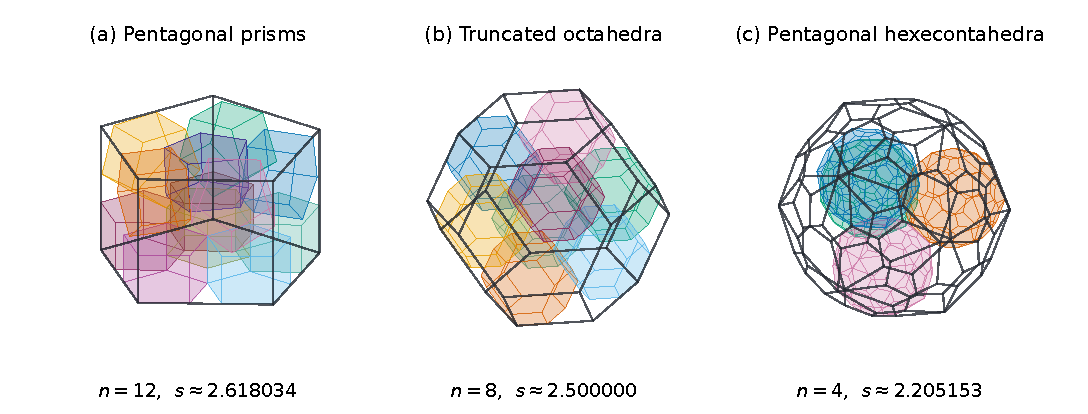
\includegraphics[width=\linewidth]{figures/generalization-examples.pdf}
\caption{Three exact-rechecked 3D witnesses from Table~\ref{tab:cases}: 12 pentagonal prisms, eight truncated octahedra and four pentagonal hexecontahedra in homothetic containers. Transparent bodies and wireframe containers show interior structure. Colors identify pieces; they do not assert distinct orientation classes. The rendering uses the native positions and rotations without spreading or altering the construction.}
\label{fig:examples}
\end{figure}

The prism and truncated-octahedron cases illustrate symmetric starts on non-tangential geometry. Their apparent contact scales $(3+\sqrt5)/2$ and $5/2$ are recorded conjectures, distinct from the slightly larger certified scales. The chiral Catalan example has 92 vertices and 60 facets per piece and requires 22,080 vertex/facet inequalities plus six separating-plane checks. Proper-rotation treatment is essential to its interpretation. The four-dimensional examples exercise native $\SO(4)$ poses and the conversion $\mu=2\sqrt2$. The eight-piece case is a nested inclusion through a 16-cell; its recorded expression $(5\sqrt2-\sqrt{10})/4$ is also only a conjectured contact limit.

The earlier patterns study~\cite{zarzueloPatterns} analyzes scale jumps and orientational domains in its smaller freeze. In the expanded setting, deletion, symmetry release and nested substitution provide specific mechanisms that can generate plateaus, orientation families and unexpectedly competitive mixed pairs. They offer explanations to test rather than proofs that the observed best constructions are optimal or that all their patterns persist to larger populations.

\subsection{A reproducible historical comparison of search moves}
We recompute the archived Round-D comparison from its six raw JSONL shards. It contains 40 cases across all 20 prism/antiprism problems then supported, with populations from 6 to 28, 1,824 valid attempts and 40,751.5 summed per-attempt elapsed seconds. The script measures elapsed wall-clock time per attempt; summing these intervals across workers does not measure processor utilization or total campaign duration. These are historical internal runs, not a new randomized or independently executed experiment. Every gain is measured against the reference scale stored in that attempt's log.

For attempts $a$ of one method, define positive logarithmic gain and gain per aggregate worker-hour by
\begin{equation}
g_a=\max\{0,\log(s_{\mathrm{ref},a}/s_a)\},\qquad
G=\frac{\sum_a g_a}{\sum_a t_a/3600}.
\end{equation}
The table reports wins using the original log's success flag, rather than silently replacing its decision rule with another tolerance. These are not matched-start comparisons: reference states and hop pools were read from an evolving archive.

\begin{table}[htbp]
\centering\small
\begin{tabular}{lrrrrr}
\toprule
Move & Attempts & Wins & Win rate & Mean seconds & $G$\\
\midrule
Fresh & 607 & 71 & 11.70\% & 25.39 & 0.2922\\
Hop & 608 & 200 & 32.89\% & 16.60 & 0.1651\\
Symmetric fresh & 609 & 86 & 14.12\% & 25.04 & 0.5446\\
\bottomrule
\end{tabular}
\caption{Recomputed Round-D outcomes. The largest improvement frequency and the largest summed improvement per aggregate worker-hour belong to different moves. Timing and archive dependence limit generalization beyond this cohort.}
\label{tab:bench}
\end{table}

Symmetric fresh starts give 3.30 times hop's and 1.86 times fresh's measured $G$, whereas hops improve the reference more often. Among 31 cases improved by more than 0.1\%, the lowest result comes from symmetric fresh in 21, fresh in five and hop in five. The evidence supports keeping distinct search mechanisms available; it does not estimate a causal benefit of temporary softening, demonstrate a fixed-budget portfolio advantage, or establish a universal speedup. There are no independent reruns or uncertainty intervals here, and Elapsed-time observations may depend on implementation, machine load and the selected historical cases.

\section{Dimension, combinatorics and computational cost}\label{sec:cost}
\subsection{One dynamics step}
Let $n$ be the piece count and $d$ the dimension. Write $V,E,F_P$ for the vertex, edge and facet counts of the active piece or eroded core, and $V_C,F_C$ for the container vertex and facet counts. Let $P_t\leq\binom n2$ be the pairs surviving the bounding-sphere test at step $t$, and $K$ the configured axis-improvement budget. The following bounds count scalar arithmetic, comparisons and elementary functions at unit cost. They concern the frozen source loops, not measured wall time or a formal execution of JavaScript, Python or numerical libraries.

A fixed-direction support query in \code{ndsim.py} walks the edge graph, accepting a vertex only when its computed value strictly increases. With finite fixed values it cannot revisit a vertex. Its trace has length at most $V$ and scans at most $2E$ adjacency entries, the graph's total degree. The Lean theorems \code{support_trace_length_le_vertices} and \code{support_neighbor_scans_le_twice_edges} prove these combinatorial statements. Including the initial value, at most $1+2E$ dot products are evaluated, giving $O(d(E+1))$ arithmetic work. A warm start can be much cheaper; a bound of merely $O(\mathrm{degree})$ for a complete query would omit the possible multiple graph hops. The positive comparison tolerance can stop short of an exact mathematical support maximum; final all-vertex certificates do not rely on that approximation.

Transforming a direction through a dense rotation costs $O(d^2)$. A new near pair receives six extra axis iterations, besides an initial gap evaluation. One higher-dimensional dynamics step, excluding optional symmetry projection, therefore has the conservative bound
\begin{equation}\label{eq:ndcost}
\begin{aligned}
O\!\bigl(&n^2d+P_t(K+7)[d^2+d(E+1)]\\
 &+nF_C[d^2+d(E+1)]+nd^3\bigr).
\end{aligned}
\end{equation}
The first term remains because the code visits every pair of centres. The wall term allows a support query at every wall, although a cheap sphere test often avoids it. Dense Cayley updates and periodic Gram--Schmidt require the cubic pose term. Optional symmetry projection adds its actual dense conjugations, currently $O(n_od^4)$ for $n_o$ orbit members, numerical SVD costs, and $O(n_fd^2g)$ for $n_f$ fixed pieces and group size $g$; these costs are not hidden in the cubic term.

The 3D engine uses separating-axis tests and closest-feature enumeration. With identical piece combinatorics there are at most $A=2F_P+E^2$ candidate axes before pruning, each requiring vertex projections. Distances between disjoint near cores can additionally inspect vertex--face and edge--edge features. For a closed convex polyhedral boundary the face--edge incidence count is $2E$. A conservative step bound is consequently
\begin{equation}\label{eq:3dcost}
\begin{aligned}
O\!\bigl(&n(V+F_P+E)+n^2+nF_CV\\
 &+P_t\{V(2F_P+E^2)+V(F_P+E)+E^2\}\bigr).
\end{aligned}
\end{equation}
Use the active core's counts for non-tangential shapes. Choosing and rebuilding a core from $H$ precomputed intervals adds $O(H+V+F_P+E)$ per step in the present implementation. Precomputing the erosion events is a separate cost.

For fixed dimension, shape and $K$, both engines retain a quadratic worst-case dependence on $n$. Increasing the piece's edge count can enlarge the 3D axis set quadratically, whereas ND queries scan an edge graph. More container facets increase wall work linearly before any solver costs. These are bounds rather than fixed multipliers for actual timings: near-pair counts, symmetry, cached directions and pruning change the observed cost.

\subsection{Dimension alone is insufficient to predict runtime}
The geometric theorem applies in every finite dimension. Explicit polytope descriptions can nevertheless grow exponentially with $d$. For $d\geq2$,
\begin{center}\small
\begin{tabular}{lccc}
\toprule
Polytope & Vertices & Edges & Facets\\
\midrule
$d$-simplex & $d+1$ & $d(d+1)/2$ & $d+1$\\
$d$-hypercube & $2^d$ & $d2^{d-1}$ & $2d$\\
$d$-orthoplex & $2d$ & $2d(d-1)$ & $2^d$\\
\bottomrule
\end{tabular}
\end{center}
Thus polynomial dependence on the explicit counts $V,E,F_C$ does not give a polynomial bound in dimension alone. Persistent ND dynamics arrays and the active problem geometry use
$O(n^2d+nF_C+nd^2+(V+V_C)d+E+F_Cd)$ scalars and indices, including the stored piece and container vertices. Optional group and orbit arrays add $O(gd^2+n)$; materializing all placed vertices adds $O(nVd)$.

\subsection{One simulation, tightening and exact verification}
For a chosen schedule of $T$ dynamics steps, the total dynamics cost is the sum of the step bounds, hence at most $T$ times a uniform step bound. The frozen fresh ND schedule specifies $\lfloor5000B\rfloor+\lfloor45000B\rfloor+\lfloor3000B\rfloor$ steps for budget multiplier $B$, before legalization. Multiple starts, retries and hops add their individual budgets. This is a finite-budget bound, without a convergence or optimality guarantee.

Tightening is separate. A container LP has $d+1$ variables and $F_C$ inequalities after support extraction; write its numerical solve cost as $T_{\rm LP}(d+1,F_C,L)$, where $L$ describes the coefficient encoding. One ND SLP round with $P$ near pairs has
\[
q=n\left(d+\frac{d(d-1)}2\right)+1+dP
\]
variables before optional regularization and at most $nVF_C+2PV$ geometric rows. Sparse row construction costs $O((nVF_C+PV)d^2+nVd^2)$, in addition to the separator, solver and legalization costs. We do not assign HiGHS a constant cost or claim a polynomial bound for the whole nonconvex search. In 3D the small-facet translation branch enumerates four active walls and checks the remaining walls, bounded by $O(F_C^5)$; the branch is used only for $F_C\leq14$. Larger containers use a capped tableau routine.

For already-expanded rational placements, direct vertex--wall and pair-projection checking uses $O(nVF_Cd+n^2Vd)$ rational arithmetic operations, in addition to source-matrix and congruence checks, with dense matrix checks bounded by $O(nd^3)$. Sparse barycentric containment of width $w$ adds $O(nVwd)$ operations and $O(nVw)$ rational coefficients. Support formulas can remove vertex enumeration from some of these tests. These operation counts are distinct from bit complexity: rational normalization and GCD costs depend on intermediate numerator and denominator sizes. They also do not bound Lean elaboration, kernel reduction or proof storage by a constant per rational operation. The recorded build receipts expose those practical costs.

The algebraic affine-basis routes have different preprocessing costs. The general 3D route's determinant enclosure explicitly sums the Leibniz formula over permutations; it is not a cubic-time elimination algorithm. With $k=d+1$ and $b$ cached bases, checking one determinant and $k^2$ adjugate entries per basis has upper bound $O(b\,k!\,k^3)$ interval operations. In contrast, the quadratic-coordinate route checks a supplied inverse by $O(bk^3)$ arithmetic operations on rational coefficient pairs, then checks its real interval enclosure. Both routes reuse caches and require $O(k^2)$ interval work for each point's weights. These are certificate-checking costs, separate from one dynamics step, inverse proposal generation, rational bit costs and kernel overhead. The arbitrary-dimensional geometric theorem does not depend on either computational representation.

\section{Limitations and testable next steps}
The generalized method changes the set of configurations that can be explored and certified, but its numerical search remains local and stochastic. Catalogue completeness over a displayed range is not exhaustive optimization. Source-only bounds and certified coordinate witnesses are distinct evidence classes. A rigorous upper bound can be worse than an uncertified contact estimate while still being the scientifically stronger feasibility statement.

A direct continuation ablation should start from the same archived hard packings, allocate the same measured budget to rigid perturbation and softening/rehardening, use identical tightening and exact acceptance rules, and reserve unseen problems for evaluation. Symmetric and crystal seeds should be compared at equal total cost, including seed construction. Outcomes should include the best certified scale, time-to-target and run-level failures, with uncertainty estimated across independently chosen seeds. The present archive and Round-D reanalysis do not replace that experiment.

Several structural hypotheses are now testable. A plateau may arise from a removable, weakly constrained piece; a sharp gain may mark a change in boundary-compatible layers or orientation domains. Symmetric starts may help when good solutions retain approximate orbits but require a small final symmetry break. Non-tangential opening may preserve useful face contacts better than uniform core scaling. Nested substitution may be especially effective when one-piece inclusions are efficient and the intermediate solid packs well. Each prediction requires comparisons against alternative constructions and compatible normalizations; none follows from visualization alone.

The Lean layer certifies actual catalogue witnesses, including their exact rigid-map representations. Extending it to every population in the archive requires further kernel builds; complete named-solid and edge-adjacency identification, and a verified parser, would also reduce the remaining external trust boundary. The present formal record comprises \leanRecords{} rational instances and \leanAlgebraicRecords{} additional algebraic-coordinate instances, alongside generic soundness theorems and separately audited computational components. It is not a proof of the entire live archive or its search software.

\section{Reproducibility and methodological tools}
The supplement contains the LaTeX source, figure-generation code, the Lean library and per-record proof sources, immutable rational-cohort inputs, proof-producing exporters, per-record build and axiom receipts, five independent production-checker rerun logs, a compressed complete catalogue snapshot, a per-case provenance CSV, the historical benchmark shards and aggregation code, and source/hash manifests. The implementation is available at \url{https://github.com/alejandrozu/platonic-packing}; the interactive catalogue is \url{https://polyhedrainpolyhedra.wiki/}. The repository commit named above freezes the computational implementation and data used here; the accompanying manuscript commit separately timestamps this document and its formal development.

The earlier DOI releases~\cite{zarzueloMethods,zarzueloPatterns,zarzueloData} remain citations to their original scope and freeze. They are not retroactive identifiers for the current 140-problem archive. Record links, \code{s_full}, geometry normalization and construction lineage should be retained when reproducing or extending an example.

Per-environment source/log archives retain the exact numerical proof sources and their build receipts without flattening independent namespaces. Original Linux build objects and raw CI artifact ZIPs are preserved separately in the repository's \href{https://github.com/alejandrozu/platonic-packing/releases/tag/lean-frozen-catalogue-2026-10-16}{proof-evidence release}, with SHA-256 indices. Preserved failed or superseded checkpoints do not contribute to verified counts. Fresh reproduction generates new local objects and receipts with the pinned toolchain.

Software tools include Python, NumPy/SciPy and numerical optimizers, JavaScript dynamics and visualization, Lean/mathlib, and LaTeX. AI coding and drafting tools, including Claude and Codex, assisted implementation, analysis and manuscript preparation under human direction. Generated suggestions are not evidence of correctness; the mathematical arguments, exact checker outputs and Lean build artifacts identify the independently inspectable support for each claim. The recorded construction credit remains distinct from software assistance.

\begin{thebibliography}{99}
\bibitem{nakajima2026} Y. Nakajima. \emph{Soft-to-Rigid: Shape Continuation as an Alternative Search for Packing Congruent Shapes}. arXiv:2610.14463v1, 2026. \url{https://arxiv.org/abs/2610.14463}.
\bibitem{zarzueloMethods} A. Zarzuelo Urdiales. \emph{Certified finite packings of Platonic solids: a generalized soft-to-rigid search and its computational development}. 2026. \url{https://doi.org/10.5281/zenodo.23306098}.
\bibitem{zarzueloPatterns} A. Zarzuelo Urdiales. \emph{Finite polyhedral fits: discrete scale jumps, orientational domains, and contact structure in 351 certified constructions}. 2026. \url{https://doi.org/10.5281/zenodo.23306126}.
\bibitem{zarzueloData} A. Zarzuelo Urdiales. \emph{Polyhedra in polyhedra packing: 351 certified constructions, structural measurements, software, and visualizations}. 2026. \url{https://doi.org/10.5281/zenodo.23306130}.
\bibitem{romanova2018} T. Romanova, J. Bennell, Y. Stoyan and A. Pankratov. Packing of concave polyhedra with continuous rotations using nonlinear optimisation. \emph{European Journal of Operational Research} 268(1), 37--53, 2018. \url{https://doi.org/10.1016/j.ejor.2018.01.025}.
\bibitem{berthold2026} T. Berthold, D. Kamp, G. Mexi, S. Pokutta and I. P\'olik. \emph{Out-of-the-Box Global Optimization for Packing Problems: New Models and Improved Solutions}. arXiv:2605.04850, 2026. \url{https://arxiv.org/abs/2605.04850}.
\bibitem{jin2015} W. Jin, P. Lu and S. Li. Evolution of the dense packings of spherotetrahedral particles: from ideal tetrahedra to spheres. \emph{Scientific Reports} 5, 15640, 2015. \url{https://doi.org/10.1038/srep15640}.
\bibitem{torquato2010} S. Torquato and Y. Jiao. Robust algorithm to generate a diverse class of dense disordered and ordered sphere packings via linear programming. \emph{Physical Review E} 82, 061302, 2010. \url{https://doi.org/10.1103/PhysRevE.82.061302}.
\bibitem{betke2000} U. Betke and M. Henk. Densest lattice packings of 3-polytopes. \emph{Computational Geometry} 16(3), 157--186, 2000. \url{https://doi.org/10.1016/S0925-7721(00)00007-9}.
\bibitem{torquato2009} S. Torquato and Y. Jiao. Dense packings of polyhedra: Platonic and Archimedean solids. \emph{Physical Review E} 80, 041104, 2009. \url{https://doi.org/10.1103/PhysRevE.80.041104}.
\bibitem{jiao2011} Y. Jiao and S. Torquato. \emph{Analytical Construction of A Dense Packing of Truncated Tetrahedra}. arXiv:1107.2300, 2011. \url{https://arxiv.org/abs/1107.2300}.
\bibitem{ping79} PingYou Ltd. Whole-body polytope inclusion construction, contribution \#79, 2026. \url{https://github.com/alejandrozu/platonic-packing/issues/79}.
\bibitem{tronford} \code{@BuilderOfAgents}/tronford. \emph{13 unit cubes in a cube: soft-to-rigid, continued}. Commit \code{c9b9b4e}, 9 October 2026. \url{https://github.com/tronford/cubes-in-cube-n13}.
\bibitem{pingConstructions} PingYou Ltd. Honeycomb windows, prism subdivision and face-lift constructions, contributions \#28, \#78 and \#85, 2026. \url{https://github.com/alejandrozu/platonic-packing/issues/28}; \url{https://github.com/alejandrozu/platonic-packing/issues/78}; \url{https://github.com/alejandrozu/platonic-packing/issues/85}.
\bibitem{archive} A. Zarzuelo Urdiales and contributors. \emph{Platonic packing: convex-polytope packing archive}. \href{\frozen}{Computational snapshot \code{1abc63218db34cea95802aeb3b6d4a6b6fe1c61b}}, 15 October 2026. \url{https://github.com/alejandrozu/platonic-packing}.
\bibitem{repoRelated} Platonic Packing project. \emph{Related work: optimization formulations for packing polytopes, dense polyhedral packings, benchmarks, and certification}. Repository literature review, 15 October 2026. \href{\blob/docs/RELATED_WORK.md}{\code{docs/RELATED_WORK.md}} at snapshot~\cite{archive}.
\bibitem{repoAudit} Platonic Packing project. \emph{Historical construction audit---13 October 2026}. Repository research note. \href{\blob/docs/HISTORICAL_SOURCE_AUDIT_2026-10-13.md}{\code{docs/HISTORICAL_SOURCE_AUDIT_2026-10-13.md}} at snapshot~\cite{archive}.
\bibitem{repoSearch} Platonic Packing project. \emph{How to search much more efficiently: literature review, our own data, and a bake-off}. Repository research note, 13 October 2026. \href{\blob/docs/SEARCH_METHODS_REVIEW.md}{\code{docs/SEARCH_METHODS_REVIEW.md}} at snapshot~\cite{archive}.
\bibitem{repoLarge} Platonic Packing project. \emph{Large n (41--100): where the time goes and how to mass-produce}. Repository research note, 14 October 2026. \href{\blob/docs/LARGE_N_REVIEW.md}{\code{docs/LARGE_N_REVIEW.md}} at snapshot~\cite{archive}.
\bibitem{repoHigher} Platonic Packing project. \emph{Higher polytopes: packing regular polytopes in 4, 5 and 6 dimensions}. Repository implementation and benchmark note, 15 October 2026. \href{\blob/docs/HIGHER_DIM.md}{\code{docs/HIGHER_DIM.md}} at snapshot~\cite{archive}.
\bibitem{stian} Stian (\code{kanin-design}). Octahedra in a cube, submitted constructions for $n=13,15,18$. Contributions \#82--84, 2026. \url{https://github.com/alejandrozu/platonic-packing/issues/82}; \href{https://github.com/alejandrozu/platonic-packing/issues/83}{\#83}; \href{https://github.com/alejandrozu/platonic-packing/issues/84}{\#84}.
\bibitem{konoha} \code{konoha-ily2}. Exact rational cube-in-cube witnesses for $n=28,34,35,36$. Contribution \#1 and associated comments, 2026. \url{https://github.com/alejandrozu/platonic-packing/issues/1}.
\bibitem{ryan} R. Xu. Cube packing coordinate records, 2026. \href{https://github.com/ry-xu/square_packing/blob/9535d65d84cc33f20f4e26329f8da12bdcef216e/cube_packing_records.json}{\code{ry-xu/square_packing}, frozen coordinate file for $n=34,35,36$}.
\bibitem{scott} S. Scott. Hyra packing audit: coordinate tightening and source comparison, 2026. \href{https://github.com/shepard5/hyra-packing-audit/tree/c107fda33c2f02df83e9d549fb839b4fd5a7bfbc}{\code{shepard5/hyra-packing-audit}, frozen audit}. Original arrangements by Haowei Lin retain their authorship.
\bibitem{builderRecon} \code{@BuilderOfAgents}/tronford. Coordinate reconstructions for 13 and 14 cubes, 2026. \href{https://github.com/tronford/cubes-in-cube-n13/tree/1f0c75401b2da4850b7e9f14de7d7b9cbe5e461a}{\code{tronford/cubes-in-cube-n13}, frozen reconstruction}. Matching historical bounds attributed to Erich Friedman.
\bibitem{hales2017} T. Hales et al. A formal proof of the Kepler conjecture. \emph{Forum of Mathematics, Pi} 5, e2, 2017. \url{https://doi.org/10.1017/fmp.2017.1}.
\bibitem{lean4} L. de Moura and S. Ullrich. The Lean 4 theorem prover and programming language. In \emph{Automated Deduction--CADE 28}, pp. 625--635, 2021. \url{https://doi.org/10.1007/978-3-030-79876-5_37}.
\bibitem{mathlib2020} The mathlib Community. The Lean mathematical library. In \emph{Certified Programs and Proofs (CPP 2020)}, pp. 367--381, 2020. \url{https://doi.org/10.1145/3372885.3373824}.
\end{thebibliography}
\end{document}
